\documentclass[10pt]{beamer}
\usetheme{jambro}

\title[]{Microeconomia I - Apresentação}
\author[]{Paulo Victor da Fonseca}
\date{28 de fevereiro de 2023}

\hypersetup{
    colorlinks = true,
    urlcolor = teal,
    linkcolor = white    
}
\usepackage[portuguese]{babel}
\usepackage{subfig}
\usepackage{emoji}

\begin{document}

\begin{frame}[plain]
    \titlepage{
        \begin{center}
            \begin{minipage}{0.8\textwidth}
                \centering
            \end{minipage}
        \end{center}}
\end{frame}

\section{Docente}
\begin{frame}{Docente}
    \begin{tabular}{cl}
        \begin{tabular}{c}
            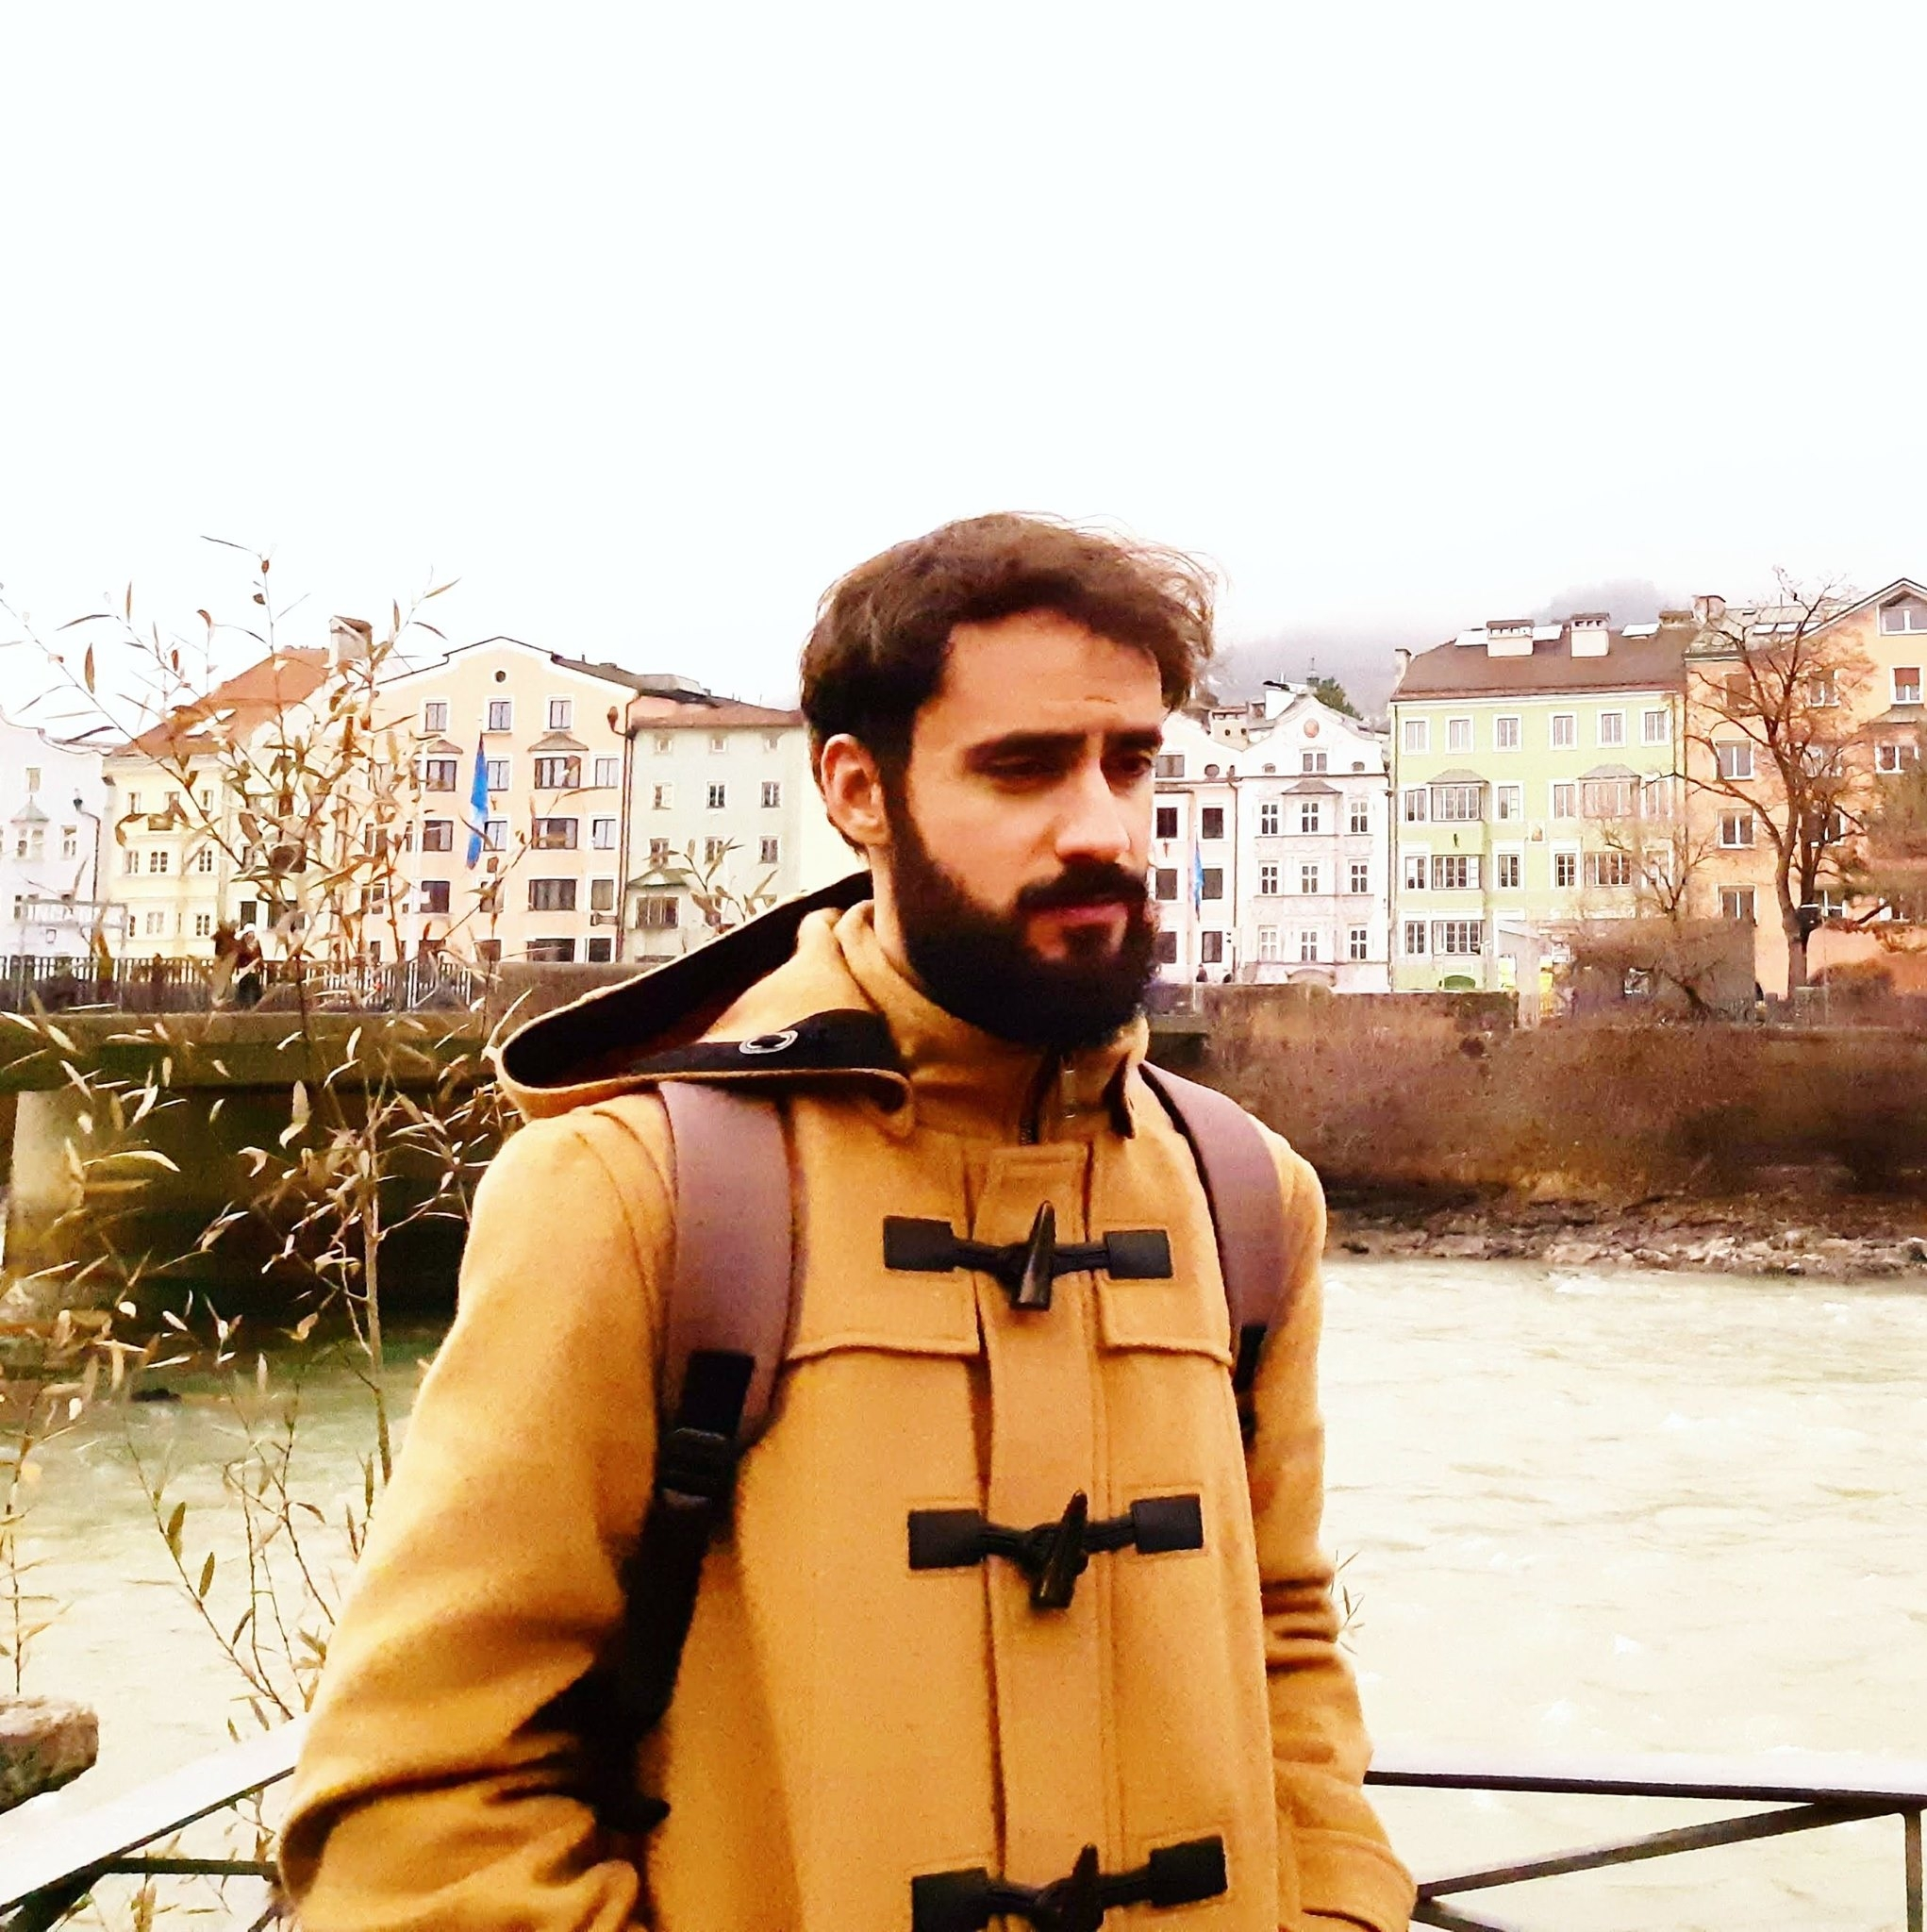
\includegraphics[width=3.5cm]{./figures/Paulo}
        \end{tabular}
         & \begin{tabular}{l}
               \parbox{0.6\linewidth}{
                   \begin{itemize}
                    \item \textbf{Nome:} Paulo Victor da Fonseca\medskip
                    \item \textbf{Formação:} Doutorado em Economia - UFSC\medskip
                    \item \textbf{Áreas de pesquisa:} Macroeconomia. Políticas monetária e fiscal. Modelos DSGE. Modelos novo-Keynesianos com agentes heterogêneos. Modelos baseados em agentes.\medskip
                    \item \textbf{Website:} \href{https://pvfonseca.github.io}{pvfonseca.github.io}\medskip
                    \item \textbf{Contato:} \href{mailto:paulo.fonseca@udesc.br}{paulo.fonseca@udesc.br}
                \end{itemize}
               }
           \end{tabular} \\
    \end{tabular}
\end{frame}

\section{Motivação}
\begin{frame}{Microeconomia I}
    \begin{itemize}
        \item A economia divide-se em dois ramos principais: microeconomia e macroeconomia. \bigskip

        \item A \tikz[tstyle]{\node[nstyle](node2){microeconomia}} trata do comportamento das unidades (agentes) econômicas individuais - e.g., consumidores, trabalhadores, proprietários de terra, empresas. \bigskip
              \begin{tikzpicture}[tpstyle]
                  \draw[pencil,very thick] ([yshift=-2pt]node2.south west) to ([yshift=-2pt]node2.south east);
              \end{tikzpicture}

        \item A microeconomia explica como e por que essas unidades tomam decisões econômicas - e.g., como consumidores tomam suas decisões de compra e como essas escolhas são influenciadas por variações nos preços e na renda.
    \end{itemize}
\end{frame}

\begin{frame}{Microeconomia I}
    \begin{itemize}
        \item Outro objeto de estudo da microeconomia é a compreensão de como as unidades econômicas (empresas) interagem para formar unidades maiores - mercados e indústrias. Por meio do estudo do comportamento e da interação entre cada empresa e os consumidores, a microeconomia revela como os setores e os mercados operam e se desenvolvem, por que são diferentes entre si e como são influenciados pelas políticas governamentais e condições econômicas globais.\bigskip

        \item Algumas questões que podem ser analisadas pelas ferramentas microeconômicas são: o aumento de um imposto qualquer, o aumento da punição de certos tipos de crimes, a liberalização das drogas, a discriminação racial, além de muitas outras.
    \end{itemize}
\end{frame}

\begin{frame}{Microeconomia I}
    A ênfase da disciplina 23MIC1 - Microeconomia I é compreender a rationale das decisões dos agentes econômicos e o propósito do curso é fornecer uma base microeconômica sólida, que será extensivamente adotada em outras disciplinas de economia. O curso será dividido em quatro blocos:\bigskip
    \begin{enumerate}
        \item Introdução \medskip
        \item Comportamento do consumidor e demanda: teoria da preferência binária \medskip
        \item Comportamento do produtor e oferta\medskip
        \item Equilíbrio parcial de mercados perfeitamente competitivos
    \end{enumerate}
\end{frame}

\section{Ementa}
\begin{frame}{Microeconomia I: Ementa}
    \begin{center}
        \begin{minipage}{.9\textwidth}
            \NB{\hlight{Teoria do consumidor:} Restrição orçamentária. Preferências do consumidor.  Comportamento do consumidor.  Demanda individual e demanda de mercado.  Elasticidade.  Preferência revelada. Equação de Slutsky.  Escolhas sob incerteza e ativos de risco. Escolha intertemporal.  Excedente do consumidor e do produtor. \medskip \\
                \hlight{Teoria da firma:} Tecnologias de produção.  Maximização de lucros.  Minimização de custos.  Curvas de custo. Oferta da empresa e oferta de mercado.
            }
        \end{minipage}
    \end{center}

\end{frame}

\section{Objetivo}
\begin{frame}{Microeconomia I: objetivo}
    \begin{center}
        \begin{minipage}{.9\textwidth}
            \NB{A disciplina apresenta os modelos básicos referentes aos comportamentos do consumidor e do produtor, que são os blocos de construção básicos da análise microeconômica contemporânea.}
        \end{minipage}
    \end{center}
\end{frame}

\section{Formato das aulas e avaliações}
\begin{frame}{Formato das aulas e sistema de avaliação}
    \begin{itemize}
        \item A disciplina apoia-se, fundamentalmente, em livros-texto e notas de aula e será ministrada por meio de aulas expositivas.\bigskip

        \item As aulas acontecerão às:\medskip
              \begin{itemize}
                  \item Terças-feiras das 08:20 às 10:00\medskip
                  \item Quintas-feiras das 10:15 às 11:55\bigskip
              \end{itemize}

        \item A avaliação será realizada a partir dos procedimentos abaixo:\medskip
              \begin{itemize}
                  \item Atividade avaliativa I (PI): 30\%\medskip
                  \item Atividade avaliativa II (PII): 30\%\medskip
                  \item Atividade avaliativa III (PIII): 20\%\medskip
                  \item Trabalhos adicionais: 20\%
              \end{itemize}
    \end{itemize}
\end{frame}

\begin{frame}{Formato das aulas e sistema de avaliação}
    \begin{itemize}
        \item Os alunos devem ter em mente que o aprendizado e o acompanhamento do curso dependem essencialmente de seu próprio esforço.\bigskip

        \item Os tópicos do programa serão apresentados em aulas expositivas, destinadas à apresentação de conceitos, modelos e suas aplicações.\bigskip

        \item[\emoji{warning}] \hlight{Embora importantes, as aulas n\~{a}o podem jamais ser vistas como substitutas da leitura regular e cuidadosa dos textos indicados e da resolu\c{c}\~{a}o dos exerc\'{i}cios propostos.}
    \end{itemize}

\end{frame}

\section{Bibliografia}

\begin{frame}{Bibliografia}
    \begin{figure}
        \centering
        \subfloat[Nicholson e Snyder (2019)\label{fig1a}]{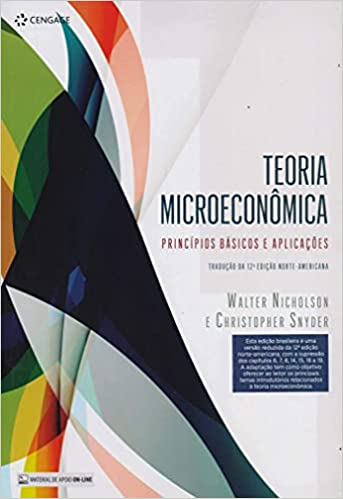
\includegraphics[width=0.23\textwidth]{./figures/nicholson}} \qquad
        \subfloat[Jehle e Reny (2011)\label{fig1b}]{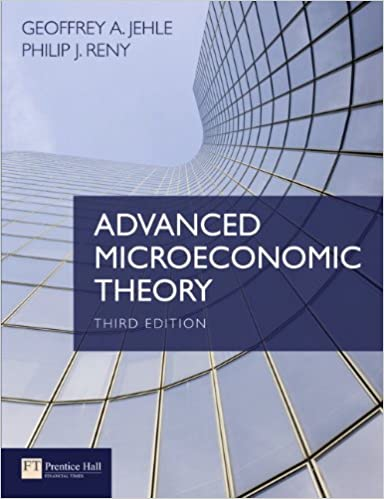
\includegraphics[width=0.25\textwidth]{./figures/jehle}} \qquad
        \subfloat[Mas-Colell et al. (1995)\label{fig1c}]{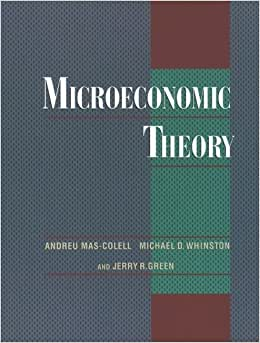
\includegraphics[width=0.25\textwidth]{./figures/colell}}
        \caption{Bibliografia do curso}
        \label{fig1}
    \end{figure}
\end{frame}

\begin{frame}{Bibliografia}
    \begin{figure}
        \centering
        \subfloat[Varian (2015)\label{fig2aa}]{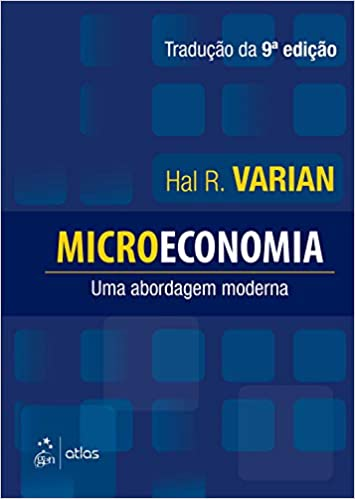
\includegraphics[width=0.24\textwidth]{./figures/varian}} \qquad
        \subfloat[Pindyck e Rubinfeld (2013)\label{fig2a}]{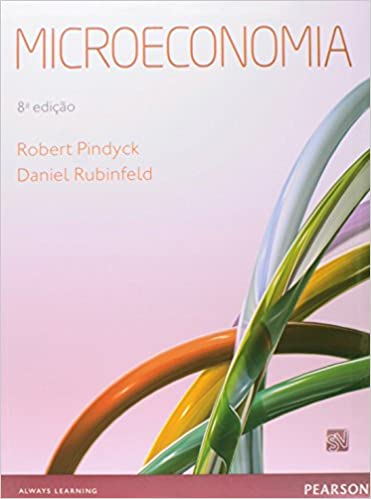
\includegraphics[width=0.25\textwidth]{./figures/pindyck}} \quad
        \subfloat[Vasconcellos et al. (2011)\label{fig2b}]{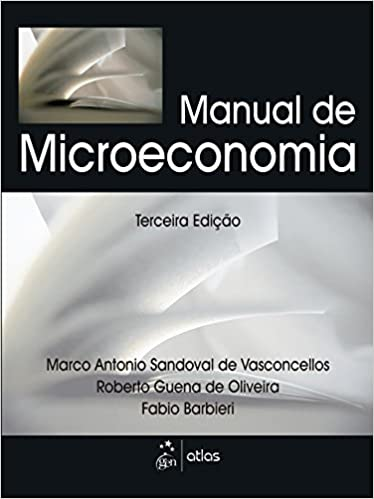
\includegraphics[width=0.25\textwidth]{./figures/vasconcellos}}
        \caption{Bibliografia do curso}
        \label{fig2}
    \end{figure}
\end{frame}

\begin{frame}{Bibliografia}
    \begin{itemize}
        \item JEHLE, G. A.; RENY, P. J. \emph{Advanced microeconomic theory}. 3.ed. Pearson Education Limited, 2011.\medskip
        \item MAS-COLELL, A.; WHINSTON, M.D.; GREEN, J.R. \emph{Microeconomic Theory}. New York, NY: Oxford University Press, 1995.\medskip
        \item NICHOLSON, W.; SNYDER C. \emph{Teoria microeconômica: Princípios básicos e aplicações}. Cengage Learning Brasil, 2019. Disponível em: \href{https://app.minhabiblioteca.com.br/books/9788522127030/}{app.minhabiblioteca.com.br/books/9788522127030}\medskip
        \item PINDYCK, R. S.; RUBINFELD, D. L. \emph{Microeconomia}. 8. ed. São Paulo: Pearson Education do Brasil, 2013.\medskip
        \item VARIAN, H. R. \emph{Microeconomia: uma abordagem moderna}. 9.ed. Rio de Janeiro: Elsevier, 2015. Disponível em: \href{https://app.minhabiblioteca.com.br/books/9788595155107}{app.minhabiblioteca.com.br/books/9788595155107}\medskip
        \item VASCONCELLOS, M. A. S.; OLIVEIRA, R. G.; BARBIERI, F. \emph{Manual de microeconomia}. 3.ed. São Paulo: Atlas, 2011. Disponível em: \href{https://app.minhabiblioteca.com.br/books/9788522469932/}{app.minhabiblioteca.com.br/books/9788522469932}
    \end{itemize}
\end{frame}
\end{document}